\chapter{Experimental Results}
This chapter gives an overview of the experimental setup, applied metrics
(\cref{sect:metrics}), and data sets (\cref{sect:staver,sect:tkstede}). Summary
and conclusion are given in \cref{sect:results-and-discussion}.

\section{Metrics}\label{sect:metrics}
To evaluate and compare approaches described in \cref{chap:Methodology} we
discuss a set of metrics in this section. We consider
\nameref{subsect:precision-recall-fscores}, \nameref{subsect:mAP} and also
introduce \nameref{subsect:normalized-iou}.

\subsection{Precision, Recall \& F-Scores}\label{subsect:precision-recall-fscores}
To the best of our knowledge, the most influential metric used in stamp 
detection is pixel-wise evaluation of the Precision and Recall
tuple~\cite{Nandedkar.2015121620151219,Younas.2017110920171115,
Ahmed.2013082520130828,Dey.2015121620151219,
Micenkova.2011091820110921, Bhalgat.16.09.2016, Micenkova.2015,
Nandedkar.2015082320150826}. Often, recall and precision are used in settings
with class imbalance where they provide a more sensible measure than accuracy.
In the stamp detection, every image pixel one can consider two classes, either
\textit{stamp} or \textit{non-stamp}. In training and evaluation images,
\textit{non-stamp}-pixels greatly outnumber \textit{stamp}-pixels. Therefore,
showing obvious class imbalance.
\par
A definition of precision and recall is given
in~\cite[423]{Goodfellow.2016} as the fraction of \textit{true} positive
detections over positive detections (i.e.\ true and false positives) and the
fraction of \textit{true} positive detections over positive \textit{datapoints}
(i.e.\ true positives and false negatives):
\begin{align}
    \text{Precision} &= \frac{t_\text{positives}}{t_\text{positives} + f_\text{positives}}\\
    \text{Recall} &= \frac{t_\text{positives}}{t_\text{positives} + f_\text{negatives}}
\end{align}
Intuitively, precision is the ``ability of a classifier to distinguish a
negative sample from [a] positive one''~\cite{Younas.2017110920171115}, while
recall is ``the ability of a classifier to classify all positive samples''~\cite{Younas.2017110920171115}.
A visual example of recall and precision is given in
\cref{fig:visual-precision-recall}.
\begin{figure}
    \center
    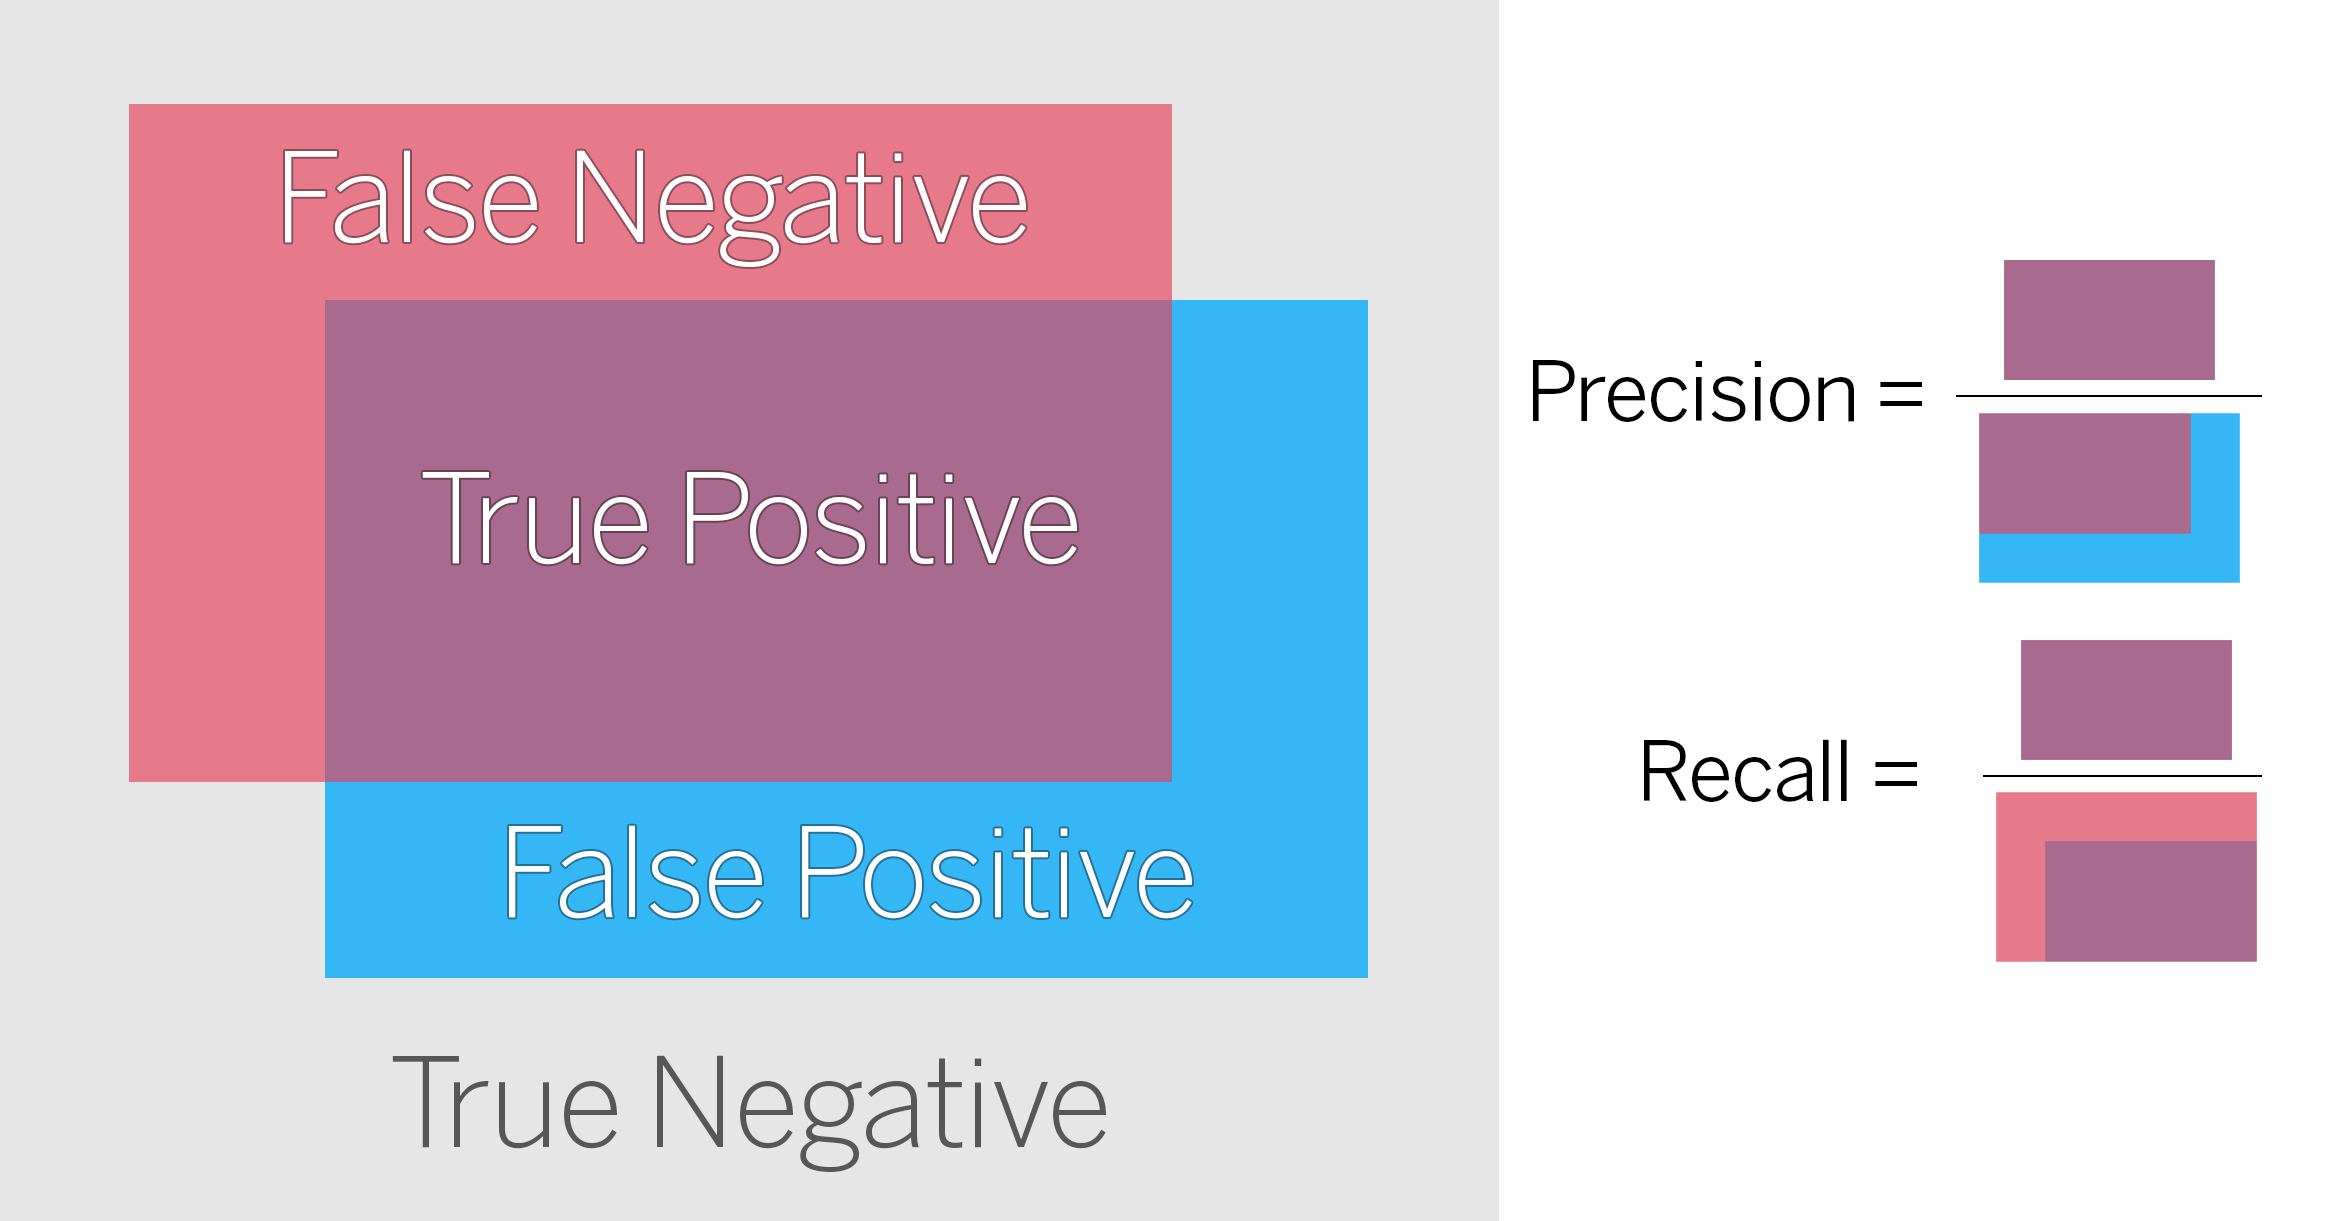
\includegraphics[width=\textwidth]{Metrics2.png}
    \caption{Visual example of recall and precision, with groundtruth (red) and
    inferred detection (blue)}\label{fig:visual-precision-recall}
\end{figure}


\subsection{Mean Average Precision}\label{subsect:mAP}
Despite its extensive use in the object detection community~\cite{Liu.2016,Ren.04.06.2015}, 
\Gls{map} was only applied in a single work \cite{Zhu.2006} from 2006. This is,
because usually ranks are not generated in most approaches, therefore the 
underlying metric of average precision, which \textit{is} computed over ranks) 
lacks meaning.

\subsection{Normalized Intersection Over Union}\label{subsect:normalized-iou}
\blindtext[1]
\todo{This kind of has the same issues as accuracy. Imagine, 99\% of images are
in the lower left corner, the a System that learns this would have a high 
average IoU. Maybe combine this from ideas of the F-Score.}

\section{StaVer}\label{sect:staver}
``The presented method is evaluated on a publicly available dataset (StaVer1) for stamp
detection and verication [sic!]. This dataset contains 400 scanned document images. Out
of these 400 documents, 80 documents contain black stamps wheras the remaining 320
documents contain colored stamps. All of these document images are available in 200,
300, and 600 dpi. For each image, two different types of ground truths are available.
One contains the pixel level ground truth, which means all of the pixels which belong to
stamps are marked in the image. The other ground truth format contains bounding box
information for each stamp. Hence, this dataset can be used for both pixel level as well
as patch level evaluation of stamp detection. In addition, it contains different types of
stamps ranging from rectangular, oval, to irregular shaped, and most importantly, textual
stamps.
For evaluation of the presented approach, the training set is generated by using 36 documents
out of 400. Out of these 36 training documents, only 6 contains black stamps
whereas the remaining 30 are with colored stamps. Testing is performed on the remaining
364 documents (74 documents with black stamps, 290 documents with colored stamps).
All the results are reported for 200 dpi documents.''~\cite{Ahmed.2016}

\section{TKStede}\label{sect:tkstede}
\blindtext[1]

\section{Results \& Discussion}\label{sect:results-and-discussion}
Goals: 
    a.) How good can stamp detection get with current frameworks
    b.) How good can classification of a vast variety of similar classes get
        with current frameworks